\documentclass[11pt,reqno]{amsart}
\usepackage{xifthen,setspace}
\usepackage{bbm}
\usepackage{esvect}
\usepackage{amsmath} % provides numberwithin (and lots more)
\usepackage{geometry}
\usepackage{graphicx}
\usepackage{caption}
\usepackage{hyperref}
\usepackage{booktabs}
\usepackage{subcaption} % Required in your preamble
\hypersetup{
    colorlinks=true,
    linkcolor=blue,
    filecolor=magenta,      
    urlcolor=cyan,
}
\usepackage{cleveref}
\geometry{a4paper, margin=0.5in}
\usepackage{lipsum}  % for sample text
%\usepackage{subfig}
% \usepackage[notcite,notref]{showkeys}
\newtheorem{assumption}{Assumption}
\newtheorem{example}{Example}
\newtheorem{defi}{Definition}
\newcommand{\lnr}{{\langle m \rangle}} 
\newcommand{\ind}{{\mathbf{1}}}
\newcommand{\vp}{{\phi}}
\newcommand{\bz}{{\bm 0}}
\newcommand{\var}{{\textrm{Var}}}
\newcommand{\eps}{{\epsilon}}
\newcommand{\p}{{\P}}
%\usepackage{refcheck} 
%\spacing{1.025}
\allowdisplaybreaks
\title[]{Milestone 3 (\href{https://github.com/Sanchayan-Bhowal/BitcoinTransactionClassification}{code link})}
\author[]{Tian Bai}
\author[]{ Sanchayan Bhowal}
\author[]{ Nathan Nguyen} 
\begin{document}
% \begin{abstract}
%     In this paper
% \end{abstract}
\maketitle

\section{Dataset overview, EDA for graph features}

We analyze FraudYelpDataset, a graph dataset classifying reviews as truthful or fraudulent. Nodes are reviews, and three edge types capture different relations: \texttt{net\_rur} (same user), \texttt{net\_rsr} (same product, same star rating), and \texttt{net\_rtr} (same product, same month). The graph has 46k nodes ($85\%$ legitimate, $15\%$ fraud), 99k \texttt{rur}, 1.1M \texttt{rsr}, and 6.8M \texttt{rtr} edges, with $32$ anonymized features per node. Table~\ref{tab:edge_homophily} reports edge-level homophily: \texttt{net\_rur} is sharply assortative (same-class probability $0.996$; fraud--fraud probability $0.91$), while the other two relations are only mildly homophilous. This asymmetry motivates treating the three relations with separate parameters.


\begin{table}[htbp]
  \centering
  \caption{Edge-level homophily by relation.}
  \label{tab:edge_homophily}
  \begin{tabular}{lrrrrrr}
    \toprule
    Relation & Num.\ edges & $P(\text{same class} \mid \text{edge type})$ & $P(\text{fraud node} \mid \text{fraud neighbor})$ \\
    \midrule
    net\_rsr & 6{,}805{,}486 & 0.7722 & 0.1857  \\
    net\_rtr & 1{,}147{,}232 & 0.7593 & 0.1764  \\
    net\_rur &      98{,}630 & 0.9964 & 0.9089\\
    \bottomrule
  \end{tabular}
\end{table}

\section{Model}

Encode the label as a spin variable $\sigma_i \in \{-1,+1\}$, with $-1$ illicit and $+1$ licit. Let $X_i \in \mathbb{R}^d$ be the node feature vector, and let $E_1, E_2, E_3$ be the three relation-specific edge sets.

\subsection{First probabilistic baseline: CAR-regularized logistic regression.}

Our first probabilistic baseline extends logistic regression, trained either on the $32$ covariates alone or with additional graph-statistics features such as $\log(1+\deg)$ and the number of fraud neighbors. Motivated by the high non-homophily of \texttt{net\_rur} edges, we use a network-regularized logistic regression model based on a conditional autoregressive (CAR) prior \cite{Brown_2018}. Specifically, we introduce a component-level lifting term $z_i^{\textsf{rur}}$ and a graph-Laplacian regularizer:
\[
\text{logit}\,\mathbb P(y_i=1)
=
\ell_i + b + \gamma z_i^{\textsf{rur}} + u_i,
\qquad
z_i^{\textsf{rur}}
=
\log\frac{\theta_i}{1-\theta_i}
-
\log\frac{\widehat \pi}{1-\widehat \pi}.
\]

Here, $\theta_i=\mathbb P(y_i=1\mid i\in C)$, where $C$ is the connected component of node $i$ under only \texttt{rur} edges. Thus, $z_i^{\textsf{rur}}$ increases the logit when the corresponding component has a high estimated fraud rate. We estimate $\theta_i$ using an Empirical Bayes Beta-Binomial estimate,
\[
\theta_i = \frac{a+k_C}{a+b+n_C},
\]
where $k_C$ and $n_C$ are the number of fraudulent nodes and total nodes in component $C$, and $a,b$ are the Beta prior parameters. We further place a Gaussian CAR prior on the residual logits
\[
u_i
=
\text{logit}\,\mathbb P(y_i=1)
-
(\ell_i+b+\gamma z_i^{\textsf{rur}}),
\]
with
\[
\pi(u)
\propto
\exp\left(
-\frac{1}{2\tau^2}u^\top(I-W)u
\right),
\]
where $W$ is the graph adjacency matrix. This gives the equivalent objective
\[
\min \ \mathrm{BCE}
+
\lambda \sum_{(i,j)\in E}(u_i-u_j)^2.
\]

This model smooths the residual logits over the graph via the Laplacian regularizer. Empirically, however, it only marginally improves over the logistic regression baseline, suggesting that it captures little additional topology beyond the edge-wise graph features already included in the baseline.

\subsection{Main model: Weighted multi-relation Ising model} 

We turn to a pairwise Markov random field \cite{daskalakis2020logistic, mukherjee2024logistic} that drops the conditional-independence assumption and lets neighboring labels be dependent. We motivate the model through a pairwise Markov random field. For a single graph $G=(V,E)$, consider
$$
    \mathbb P(\sigma_1,\ldots,\sigma_n\mid X,G)
    \propto
    \prod_{(i,j)\in E}
    \psi_{X_i,X_j}(\sigma_i,\sigma_j).
$$
Since $\sigma_i,\sigma_j\in\{-1,+1\}$, any symmetric pairwise log-potential
can be written as
$$
    \log \psi_{X_i,X_j}(\sigma_i,\sigma_j)
    =
    \beta_{ij}\sigma_i\sigma_j
    +
    \alpha_{ij}(\sigma_i+\sigma_j)
    +
    c_{ij}.
$$
%% Equivalently,
% $$
    % \psi_{X_i,X_j}(\sigma_i,\sigma_j)
    % =
    % \exp\left\{
    % \beta_{ij}\sigma_i\sigma_j
    % +
    % \alpha_{ij}(\sigma_i+\sigma_j)
    % +
    % c_{ij}
    % \right\}.
% $$
The interaction term $\beta_{ij}\sigma_i\sigma_j$ captures dependence between
neighboring labels. If $\beta_{ij}>0$, adjacent labels prefer to agree; if
$\beta_{ij}<0$, adjacent labels prefer to disagree. The terms
$\alpha_{ij}(\sigma_i+\sigma_j)$ contribute to node-level external fields.

A single global $\beta$ is too restrictive given the homophily gap in Table~\ref{tab:edge_homophily}, so we use one coupling $\beta_r$ per relation. We further argue that even within a relation, edges should not be weighted equally: connected nodes with similar features ought to influence each other more than dissimilar ones. Therefore, we introduce the RBF kernel to model similarity-weighted interaction, defined as follows, for $(i,j) \in E_r$, let $w_{ij}^{(r)}$ be the feature-similarity weight 

\[w_{ij}^{(r)} = w_{ij}^{(r)}
    =
    \exp\left(
    -\frac{\|X_i-X_j\|_2^2}{2\tau_r^2}
    \right),\]
where $\tau_r > 0$ is a bandwidth hyperparameter for relation $r$. 
This leads to the weighted interaction model
$$
    \mathbb P_{\beta,\theta}(\sigma\mid X,G_1,G_2,G_3)
    \propto
    \exp\left\{
    \sum_{r=1}^3
    \beta_r
    \sum_{(i,j)\in E_r}
    w_{ij}^{(r)}\sigma_i\sigma_j
    +
    2\sum_{i=1}^n\sigma_i X_i^\top\theta
    \right\}.
$$


To prevent high-degree nodes from dominating, we normalize by the weighted degree $D_i^{(r)} = \sum_k A_{ik}^{(r)} w_{ik}^{(r)}$, 

\[
    \mathbb P_{\beta,\theta}(\sigma\mid X,G_1,G_2,G_3)
    \propto
    \exp\left\{
    \sum_{r=1}^3
    \beta_r
    \sum_{i=1}^n
    \sum_{j=1}^n
    A_{ij}^{(r)}w_{ij}^{(r)}
    \left(
    \frac{1}{D_i^{(r)}}+\frac{1}{D_j^{(r)}}
    \right)
    \sigma_i\sigma_j
    +
    2\sum_{i=1}^n \sigma_i X_i^\top\theta
    \right\}.
\]

Finally, we replace the linear external field $X_i^\top\theta$ with a scalar function $b_\theta(X_i)$, instantiated either as $X_i^\top\theta$ (linear) or as an MLP (neural). The full model is


$$
    \mathbb P_{\beta,\theta}(\sigma\mid X,G_1,G_2,G_3)\propto\exp\left\{\sum_{r=1}^3\beta_r\sum_{(i,j)\in E_r}w_{ij}^{(r)}\sigma_i\sigma_j+2\sum_{i=1}^n\sigma_i b_\theta(X_i)\right\}.
$$

We refer to the two variants as \texttt{hm\_weighted\_linear} and \texttt{hm\_weighted\_nn}. This formulation preserves the original network-regularized logistic idea while adapting it to a multi-relation graph, similarity-weighted edges, degree normalization, and nonlinear covariate effects.

\section{Model Implementation}

The partition function of the full joint sums over $2^n$ configurations and is intractable, so we estimate parameters by \emph{pseudo-maximum likelihood}: we replace the joint by the product of node-wise conditionals, conditioning only on observed training labels $\sigma^{\text{obs}}$ (validation and test labels are held out). Define the local field
\[
h_i \;=\; \sum_{r=1}^{3} \beta_r \sum_{j} A_{ij}^{(r)} w_{ij}^{(r)}
\!\left(\frac{1}{D_i^{(r)}} + \frac{1}{D_j^{(r)}}\right)\!
\sigma_j^{\text{obs}}
\;+\; 2\, b_\theta(X_i).
\]

Each conditional reduces to a logistic form $\mathbb{P}(\sigma_i \mid \cdot) = e^{\sigma_i h_i}/(2\cosh h_i)$, giving the negative pseudo-log-likelihood
\[
\mathcal{L}(\beta, \theta) \;=\; \frac{1}{|\mathcal{T}|} \sum_{i \in \mathcal{T}} \bigl[\log(2\cosh h_i) \;-\; \sigma_i h_i\bigr].
\]
We minimize $\mathcal{L}$ jointly over $\beta = (\beta_1, \beta_2, \beta_3)$ and $\theta$ with AdamW and backpropagation. We track validation F1 and AUPRC each epoch and use early stopping on validation F1. The classification threshold $t$ is also tuned on the validation set. $b_\theta(X_i) = X_i^\top \theta$ for linear model, or a general neural network. 

\section{Prediction and Evaluation}

After training, the fitted probability that node $i$ has label $+1$ is
$$
    \widehat{\mathbb P}(\sigma_i=+1\mid X,G_1,G_2,G_3,\sigma_{\mathrm{obs}})
    =
    \operatorname{logit}^{-1}
    \left[
    2\left(
    \sum_{r=1}^3
    \widehat\beta_r
    A_{ij}^{(r)}w_{ij}^{(r)}
    \left(
    \frac{1}{D_i^{(r)}}+\frac{1}{D_j^{(r)}}
    \right)
    \sigma_j^{\mathrm{obs}}
    +
    2b_{\widehat\theta}(X_i)
    \right)
    \right].
$$
With our sign convention, this is the fitted probability that node $i$ belongs to the licit class.

A binary prediction is obtained by thresholding this probability:
$$
    \widehat\sigma_i
    =
    \begin{cases}
        +1, & \text{if }
        \widehat{\mathbb P}(\sigma_i=+1\mid X,G_1,G_2,G_3,\sigma_{\mathrm{obs}})\ge t, \\
        -1, & \text{otherwise.}
    \end{cases}
$$
Since the classes are imbalanced, the default threshold $t=0.5$ may not be optimal. We choose $t$ using the validation set, for example by maximizing validation F1-score or validation balanced accuracy. Figure~\ref{fig:f1} compares the final F1-scores across a range of different models and calibration strategy. We see that \texttt{hm\_weighted\_nn}, the neural net version of our model, achieves overall competitive performance. The simpler model using linear regression, named \texttt{hm\_weighted\_linear}, is less predictive compared to the more powerful neural version but can still outperform most baseline models such as GCN or GAT.

For a comprehensive compairson, we also evaluate the model using ROC-AUC and average precision, which are threshold-independent metrics. We also report accuracy, precision, recall, F1-score, and balanced accuracy at the selected threshold. Average precision and F1-score are especially relevant because the illicit class is rare.
A summary of the model performance metrics is presented in Figure~\ref{fig:heatmap}.

\begin{figure}[ht]
    \centering

    \begin{subfigure}[t]{0.58\textwidth}
        \centering
        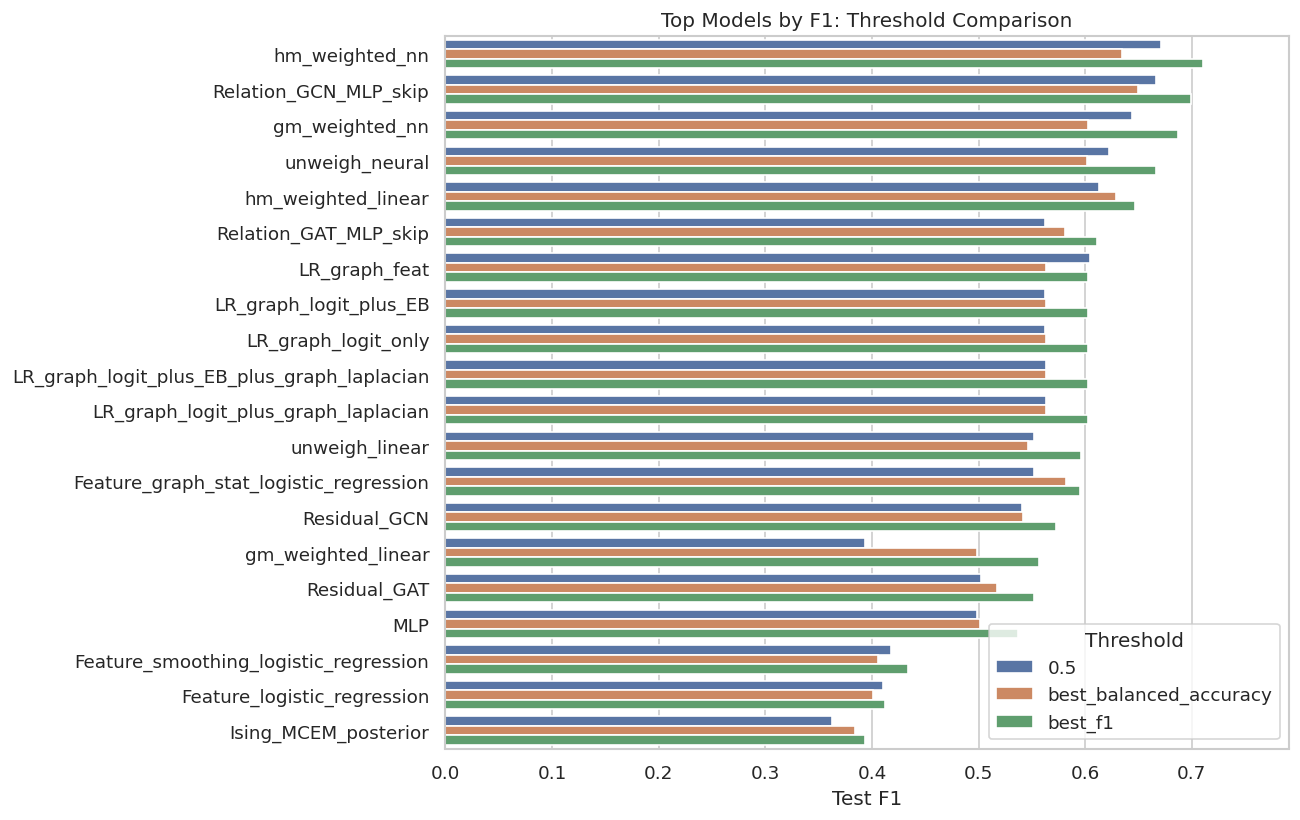
\includegraphics[width=\textwidth]{figures/fraud_yelp/f1.png}
        \caption{F1-score comparison across models.}
        \label{fig:f1}
    \end{subfigure}
    \hfill
    \begin{subfigure}[t]{0.38\textwidth}
        \centering
        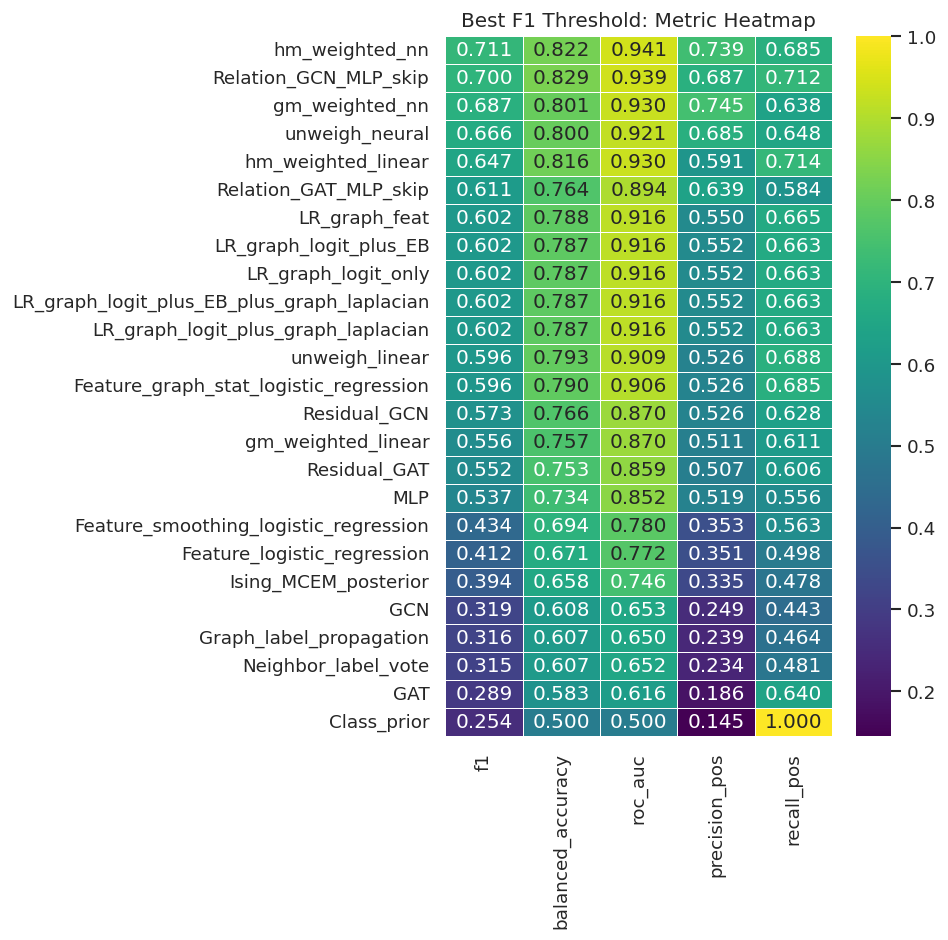
\includegraphics[width=\textwidth]{figures/fraud_yelp/metrics_heatmap.png}
        \caption{Metrics heatmap across models.}
        \label{fig:heatmap}
    \end{subfigure}

    \caption{FraudYelp model performance comparison.}
    \label{fig:fraud_yelp_results}
\end{figure}

To understand which edge types are more predictive, we inspect the fitted coefficients
$$
    \widehat\beta_1,\widehat\beta_2,\widehat\beta_3.
$$
A large value of $|\widehat\beta_r|$ indicates that relation $r$ has a strong graph effect after controlling for node features. A positive coefficient indicates assortative behavior, while a negative coefficient indicates disassortative behavior.

Since the three graph covariates may still have different empirical scales, we also use ablation experiments. We remove one edge type at a time, refit the model, and compare validation and test performance. If removing relation $r$ causes a large drop in F1-score, balanced accuracy, or average precision, then relation $r$ contains substantial predictive information.

\bibliographystyle{plain}
\bibliography{refs}

\section*{AI Disclosure}
We used AI tools to locate relevant data sources and to clarify certain definitions that we were unfamiliar with. We also used AI assistance for minor grammar corrections and sentence rephrasing, as well as shortening our report to appropriate length. We also use AI to suggest for some modeling refinements in the graph-Laplacian CAR models as well as identifying relevant literature, yet the original idea is not generated by AI For CAR model, we also use AI to double check original implementation for EDA and models, but the analysis and ablation idea are original work. We verify carefully the results by sanity-checking the AI suggestions. 

For main model and analysis, we design the original codebase and used AI to assist with better code generation and optimization. We verify carefully the results by sanity-checking the AI suggestions. All substantive content, including the ideas, modeling, and analysis presented in this work, is our own and was not generated by AI.
\end{document}
